\documentclass[final,hyperref={pdfpagelabels=false}]{beamer}
\mode<presentation>
\usepackage{color}
\usepackage[size=custom,width=36,height=36,scale=.8,orientation=portrait]{beamerposter}

\setbeamertemplate{navigation symbols}{}
\usetheme{SICM}

\definecolor{plotblue}{cmyk}{1,1,0,0}
\definecolor{plotgreen}{cmyk}{1,0,1,0.5}
\definecolor{plotred}{cmyk}{0,1,1,0}
\definecolor{plotyellow}{cmyk}{0,0.35,1,0}

\title{Simplified Interface to Complex Memory}
\author{Sean Williams, PhD}
\institute{Los Alamos National Laboratory}
\date{}

\begin{document}
\begin{frame}{}
\begin{columns}[t]
  \begin{column}{.45\linewidth}
    \begin{block}{Problem}
      \begin{itemize}
        \item Exascale nodes expected to have complex, heterogeneous memory systems
        \item Users won't want to learn low-level technical details
        \item Heterogeneity is the enemy of portability
        \item Middleware requries unified low-level abstraction
      \end{itemize}
    \end{block}
    
    \begin{block}{Proposed Solution}
      Two-level library:
      \begin{itemize}
        \item Low-level interface:
        \begin{itemize}
          \item Homogeneous abstraction over different memory devices
          \item Classifies devices according to designer intent
          \item Unified method of querying, allocating, and freeing
          \item Intended for advanced users or middleware developers
        \end{itemize}
        \item High-level interfaces:
        \begin{itemize}
          \item Expose memory systems in intentional terms, rather than technical
          \item Choose where to allocate, when to migrate
          \item Many possible implementations
          \item Basis for other research into memory management
        \end{itemize}
      \end{itemize}
    \end{block}
    
    \begin{block}{Project Team}
      Point of Contact: Mike Lang (mlang@lanl.gov) \\
      \small
      Roger Pearce (pearce7@llnl.gov) \\
      Maya Gokhale (gokhale2@llnl.gov) \\
      Simon Hammond (sdhammo@sandia.gov) \\
      Sean Williams (swilliams@newmexicoconsortium.org) \\
      Douglas Otstott (douglas.otstott@gmail.com) \\
      Latchesar Ionkov (lionkov@lanl.gov) \\
      Ada Gavrilovska (ada@cc.gatech.edu) \\
      Greg Eisenhauer (eisen@cc.gatech.edu) \\
      Thaleia-Dimitra Doudali (doudali@gmail.com) \\
      Terry Jones (trjones@ornl.gov) \\
      Aaron Welch (welchda@ornl.gov) \\
      Benjamin Mayer (mayerbw@ornl.gov) \\
      Saurabh Hukerikar (hukerikarsr@ornl.gov)
    \end{block}
  \end{column}
  
  \begin{column}{.45\linewidth}
    \begin{block}{Preliminary Results}
      Early low-level interface:
      \begin{itemize}
        \item Currently provides abstraction over NUMA nodes, page size, and Intel Knights Landing high-bandwidth memory
        \item Written in C, with FORTRAN bindings
      \end{itemize}
      Added support to a proxy application:
      \begin{itemize}
        \item We use SNAP, a proxy particle transport simulation
        \item Tested NUMA pinning and huge pages
      \end{itemize}
      Results:
      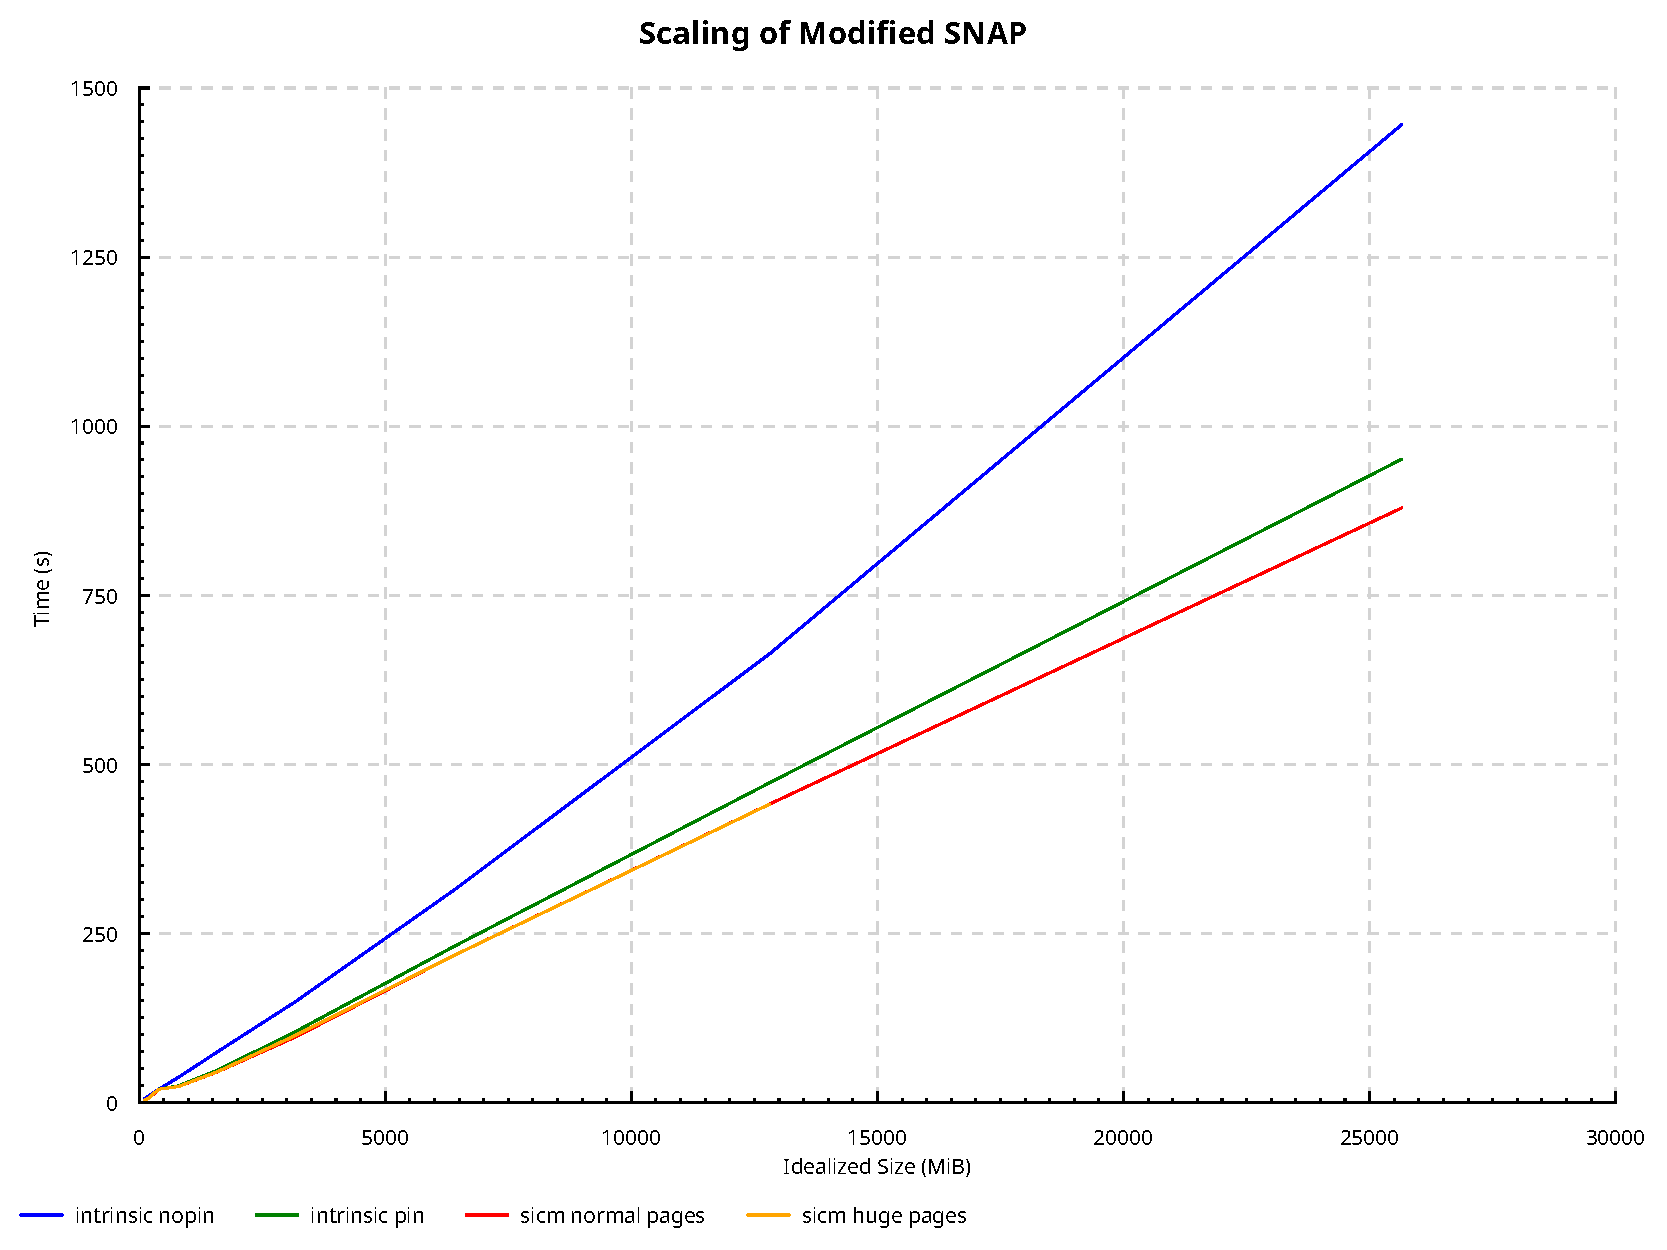
\includegraphics[width=\textwidth]{snap.pdf}
      \begin{itemize}
        \item \textcolor{plotblue}{Normal run, allocations with FORTRAN \texttt{ALLOCATE}}
        \item \textcolor{plotgreen}{Pin to single NUMA node, uses \texttt{ALLOCATE}}
        \item \textcolor{plotred}{Pin to single NUMA node, uses SICM}
        \item \textcolor{plotyellow}{Pin to single NUMA node, huge pages with SICM}
      \end{itemize}
    \end{block}
    
    \begin{block}{Repository}
      https://github.com/lanl/SICM
    \end{block}
  \end{column}
\end{columns}
\end{frame}
\end{document}
